%% Submissions for peer-review must enable line-numbering 
%% using the lineno option in the \documentclass command.
%%
%% Camera-ready submissions do not need line numbers, and
%% should have this option removed.
%%
%% Please note that the line numbering option requires
%% version 1.1 or newer of the wlpeerj.cls file, and
%% the corresponding author info requires v1.2

\documentclass[fleqn,10pt,lineno]{wlpeerj}

\usepackage{amsmath,amssymb,amsthm}
\usepackage{booktabs,tabularx,array}
\usepackage{natbib}
\usepackage{url}
\usepackage{listings}
\usepackage{orcidlink}
\usepackage{graphicx}
\usepackage{xspace} % Added for robust macro spacing

\newtheorem{definition}{Definition}
\newtheorem{proposition}{Proposition}
\newtheorem{remark}{Remark}

\newcolumntype{Y}{>{\raggedright\arraybackslash}X}
\newcommand{\PASS}{\mathsf{PASS}}
\newcommand{\FAIL}{\mathsf{FAIL}}
\newcommand{\Active}{\mathsf{ACTIVE}}
\newcommand{\Spent}{\mathsf{SPENT}}
\newcommand{\Auth}{\mathsf{Authorized}}
\newcommand{\Released}{\mathsf{Released}}
\newcommand{\Refunded}{\mathsf{Refunded}}
\newcommand{\enc}{\operatorname{encode}}
\newcommand{\Eval}{\operatorname{Eval}}
\newcommand{\JCS}{\operatorname{JCS}}
\newcommand{\Hash}{\operatorname{SHA256}}
\newcommand{\ualgo}{\ensuremath{\mu\mathrm{ALGO}}\xspace} % Fixed with xspace

\title{T-REX: Syntactic Predicate-Conditioned Threshold-Attested
Settlement and AVM Budget Management for HTTP-Native Agentic Commerce}

\author[1]{Minh Tuan Le}

\affil[1]{Faculty of Electrical and Electronics Engineering, Hanoi Open University, Hanoi 10000, Vietnam}
\corrauthor[1]{Minh Tuan Le}{lmtuan@hou.edu.vn}

\begin{abstract}
\textbf{Background:} HTTP-native payments facilitate automated service procurement, yet payment authorization, response evidence validation, and conditional fund release remain fundamentally decoupled. T-REX rigorously integrates these operations for syntactic service conditions under an explicitly permissioned attestation model.
\textbf{Methods:} The protocol commits an HTTP request and a restricted JSON predicate at authorization, binds a response commitment to seller and attester signatures, and executes release or refund transitions via an Algorand application. A 2-of-3 registered quorum evaluates predicates off-chain using a strict fail-closed logical framework. Buyer-signature verification occurs during authorization, while terminal verification leverages pooled AVM budgets to optimize L1 execution costs.
\textbf{Results:} The unified hardened artifact (App 772170811) successfully validated 100 functional Testnet sessions and rejected 10 targeted adversarial mutations. Historical profiling demonstrates settlement and attested-fail refund groups requiring 6,730 and 4,511 cost units, comfortably accommodated within pooled budgets of 7,000 and 4,900 units. The optimized deployment configuration utilizes 22 outer and two inner transactions per normal session, costing 24,000~\ualgo at the stated fee rate. Aggregate timing metrics for 40 normal sessions yield a mean client-observed RPC round-trip time of 9.87 seconds.
\textbf{Conclusions:} The empirical results definitively support the architectural feasibility and security invariants of the T-REX protocol. The strict separation of abstract safety arguments, empirical functional validation, and analytical cost calculations establishes a reproducible baseline for HTTP-native agentic settlement layers.
\end{abstract}

\begin{document}

\flushbottom
\maketitle
\thispagestyle{empty}

% ============================================================
\section{Introduction}
Automated buyers can procure API responses without a human approving each interaction \citep{lcta,CPMMHuang2026}. An HTTP payment exchange must nevertheless rigorously distinguish authorization to spend, the response presented as evidence, and the decision to release funds. HTTP reserves status code 402 for payment use, and x402 develops an application-level payment workflow around it \citep{HTTP9110,x402}. These mechanisms motivate a critical engineering imperative: how can a constrained smart-contract platform settle a payment according to an explicitly agreed, machine-evaluable response condition without introducing off-chain trust assumptions?

Existing mechanisms cover isolated facets of this problem. Signed offers and receipts provide portable interaction evidence, while x402r auth-capture supports escrow, capture, void, refund, and deadline-based reclaim \citep{x402_ext,X402EscrowSpec}. Conditional exchange and verifiable service-payment protocols also predate T-REX \citep{asokan2004,rcsp}. Rather than reinventing foundational escrow primitives, our core contribution is the rigorous integration of these components into a scoped request--predicate--response settlement workflow, coupled with an explicit optimization of Algorand Virtual Machine (AVM) resource constraints. Figure~\ref{fig:x402_standard} provides context for distinguishing payment authorization from service-response evidence. The central question addressed here is how to cryptographically bind a committed syntactic predicate and threshold-attested response evidence to a unique, replay-resistant terminal payment transition.

T-REX (Triple-entry Receipt Exchange) leverages a permissioned B2B consortium to attest whether a JSON response satisfies a restricted predicate. The blockchain verifies commitments and signatures; it does not parse the semantic utility of the response. This strict separation of syntactic validation from semantic truth is the cornerstone of both the security model and the empirical evaluation presented herein.

\subsection{Research questions and contributions}

The study addresses four core questions:

\begin{enumerate}
\item How can a session cryptographically bind buyer authorization, a request, a predicate, response evidence, and a unique terminal payment transition?
\item What signature-verification decomposition optimally fits constrained AVM budgets, and how do execution budgets and transaction fees interact?
\item Which assumptions guarantee safety and eventual termination, and how are these properties empirically validated?
\item What settlement evidence schema can support downstream audit and accounting workflows without automating subjective accounting recognition?
\end{enumerate}

The primary contributions are: (1) a protocol specification with typed commitments and explicit terminal guards; (2) a fail-closed off-chain predicate language with defined error semantics; (3) conditional safety and liveness proofs; (4) a configuration-specific AVM and fee analysis demonstrating the necessity of budget pooling; and (5) an evidence schema linking authorization and settlement to downstream records. Crucially, the evaluation strictly partitions results by application artifact, ensuring that historical development data is never conflated with final security validations.

\begin{figure}[htbp]
\centering
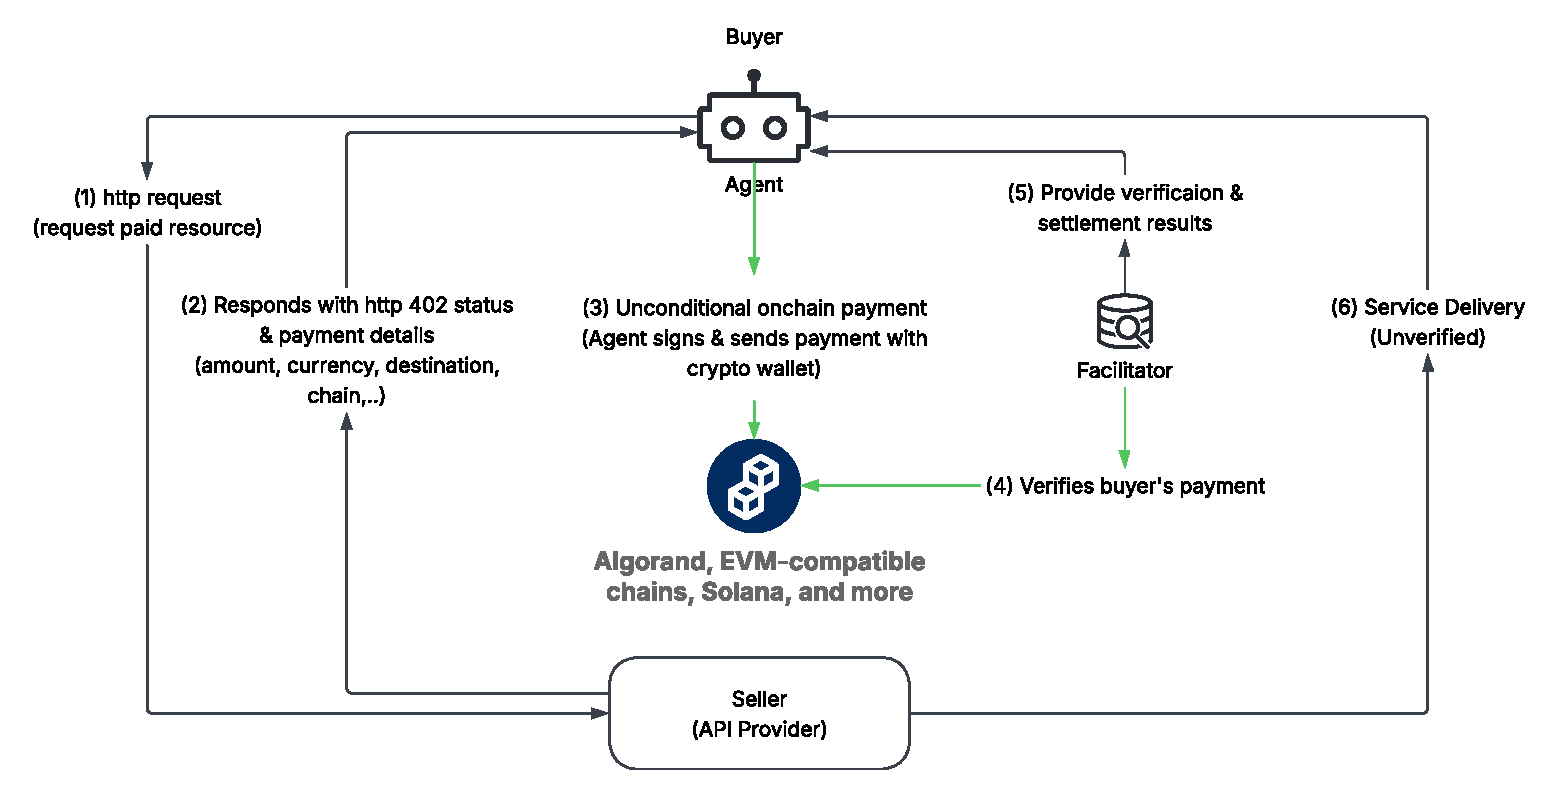
\includegraphics[width=\columnwidth]{Fig1.pdf}
\caption{The standard x402 authorization and escrow flow. The architecture exposes a structural gap where service delivery remains unverified and decoupled from settlement finality (green: on-chain, black: off-chain).}
\label{fig:x402_standard}
\end{figure}

% ============================================================
\section{Background and related work}
% ============================================================

\subsection{HTTP payment and service evidence}

The x402 offer/receipt extension signs payment terms and interaction records. The x402r auth-capture scheme additionally allows authorization before resource delivery and later capture or return of funds \citep{x402_ext,X402EscrowSpec}. T-REX specializes the decision rule through a committed predicate and registered attestations. It is an HTTP-oriented settlement design; wire-level interoperability requires a separately specified adapter.

The analysis by \citet{li2026five} identifies revert-grant, settlement preemption, replay/idempotency, header/proxy confusion, and server-selection attacks. Session binding and terminal-state checks in T-REX definitively neutralize settlement-layer failure modes and replay attacks, though they do not repair HTTP caching or discovery manipulations. 

A402 studies payment--execution binding using atomic service channels and trusted execution mechanisms \citep{A402Li2026}. RC-S-P formalizes recurring payment for verifiable services \citep{rcsp}. An HTLC conditions transfer on a preimage and a deadline \citep{htlc}, but lacks the capability to evaluate complex JSON predicates. The Lightning Network uses payment channels to support off-chain payments \citep{LightningPoonDryja2016}. These fundamental differences in trust assumptions and verification mechanisms motivate capability-aware comparisons rather than superficial fee benchmarks.

\subsection{Shared evidence and accounting}

Boyle's discussion of general-ledger architecture distinguishes shared transaction records from entity-specific reporting functions \citep{boyle2001}. Triple-entry accounting motivates a shared, verifiable record connecting counterparties' records \citep{grigg2005,Cai2019,tea_slr1}. Blockchain-based accounting research distinguishes ledger evidence from broader assurance and reporting responsibilities \citep{DaiVasarhelyi2017}.

Related surveys examine blockchain-based triple-entry accounting in B2B settings \citep{tea_slr2} and map the broader accounting literature \citep{BlockchainAccountingReview2026}. At the protocol level, \citet{pan2023} propose a private triple-entry accounting protocol on Bitcoin. These studies provide the ledger-design context for the ``third entry'' in T-REX: a shared, immutable record anchoring a settlement event. T-REX provides the cryptographic evidence layer; it neither replaces double-entry bookkeeping nor automates IFRS 15 revenue recognition.

\subsection{AVM execution and fees}

Algorand's consensus design provides the blockchain foundation \citep{AlgorandMicali2017,gilad2017}. Its smart-contract environment supports atomic transaction groups and budgeted application calls \citep{algorand_costs}. For the evaluated TEAL v11 configuration, each outer application call contributes 700 cost units to the pooled application budget. Both \texttt{ed25519verify} and \texttt{ed25519verify\_bare} cost 1,900 units \citep{AlgorandOpcodeRef}. OpUp-style calls obtain additional execution budget using existing platform facilities; T-REX leverages this mechanism to amortize cryptographic costs across atomic groups \citep{pyteal_opup}. Execution units, transaction fees, escrow principal, and minimum-balance requirements are strictly accounted for as orthogonal vectors.

% ============================================================
\section{System and threat model}
% ============================================================

\subsection{Participants and boundaries}

The participants are a buyer $B$, a seller $S$, three registered attesters $A_1,A_2,A_3$, a relayer $R$, and an Algorand application. The buyer authorizes a payment and funds escrow. The seller supplies a response and signs its commitment. Attesters evaluate the agreed predicate over the selected response. A relayer submits a terminal call and receives a funded bounty upon success.

The attester set is permissioned. Distinct keys do not establish organizational independence. Cryptographic provenance mechanisms such as DECO \citep{deco}, zkTLS \citep{zktls}, and TLSNotary \citep{tlsnotary} may support a stronger future evidence path, but do not by themselves establish semantic service quality.

An adversary may control a buyer or seller, manipulate network delivery, operate relayer identities, and compromise at most one attester. The classical Dolev--Yao framework provides background for reasoning about adversarial message manipulation \citep{DolevYao1983}. The arguments below rely on the explicit cryptographic and operational assumptions A1--A5. Safety does not require timely delivery. Liveness additionally requires the availability assumptions stated below.

\paragraph{Collusion and Sybil boundaries.} 
The 2-of-3 threshold model inherently assumes economic and operational independence among attesters. T-REX does not cryptographically prevent a scenario where a Byzantine attester colludes with or is bribed by the seller to sign a fraudulent $\mathsf{PASS}$ verdict. Mitigating off-chain quorum collusion requires external reputation systems or stake-slashing mechanisms, which remain outside the scope of the current on-chain settlement layer.

\subsection{Assumptions}

\begin{enumerate}
\item[\textbf{A1.}] Ed25519 signatures are unforgeable under the adopted key-management model \citep{Brendel2021}, the commitment hashes resist collisions, and the encoding is unambiguous \citep{RFC8032,NISTFIPS1804}.
\item[\textbf{A2.}] The ledger preserves atomic execution and finality. Eventual inclusion of valid transactions is assumed only when deriving liveness.
\item[\textbf{A3.}] At most one registered attester is Byzantine. Honest attesters use the same evaluator and agreed response-selection policy.
\item[\textbf{A4.}] The relevant contract policy remains fixed: stored session terms, the attester set, bounty, and terminal routing cannot be changed during a session.
\item[\textbf{A5.}] For liveness, at least one funded submitter observes the session, can construct a valid transaction, and eventually submits it.
\end{enumerate}

Two quorums of size two can intersect only in a Byzantine attester. Under A3, each accepted quorum contains an honest signature over the agreed input.

% ============================================================
\section{Protocol specification}
\label{sec:protocol}
% ============================================================
\begin{figure}[htbp]
\centering
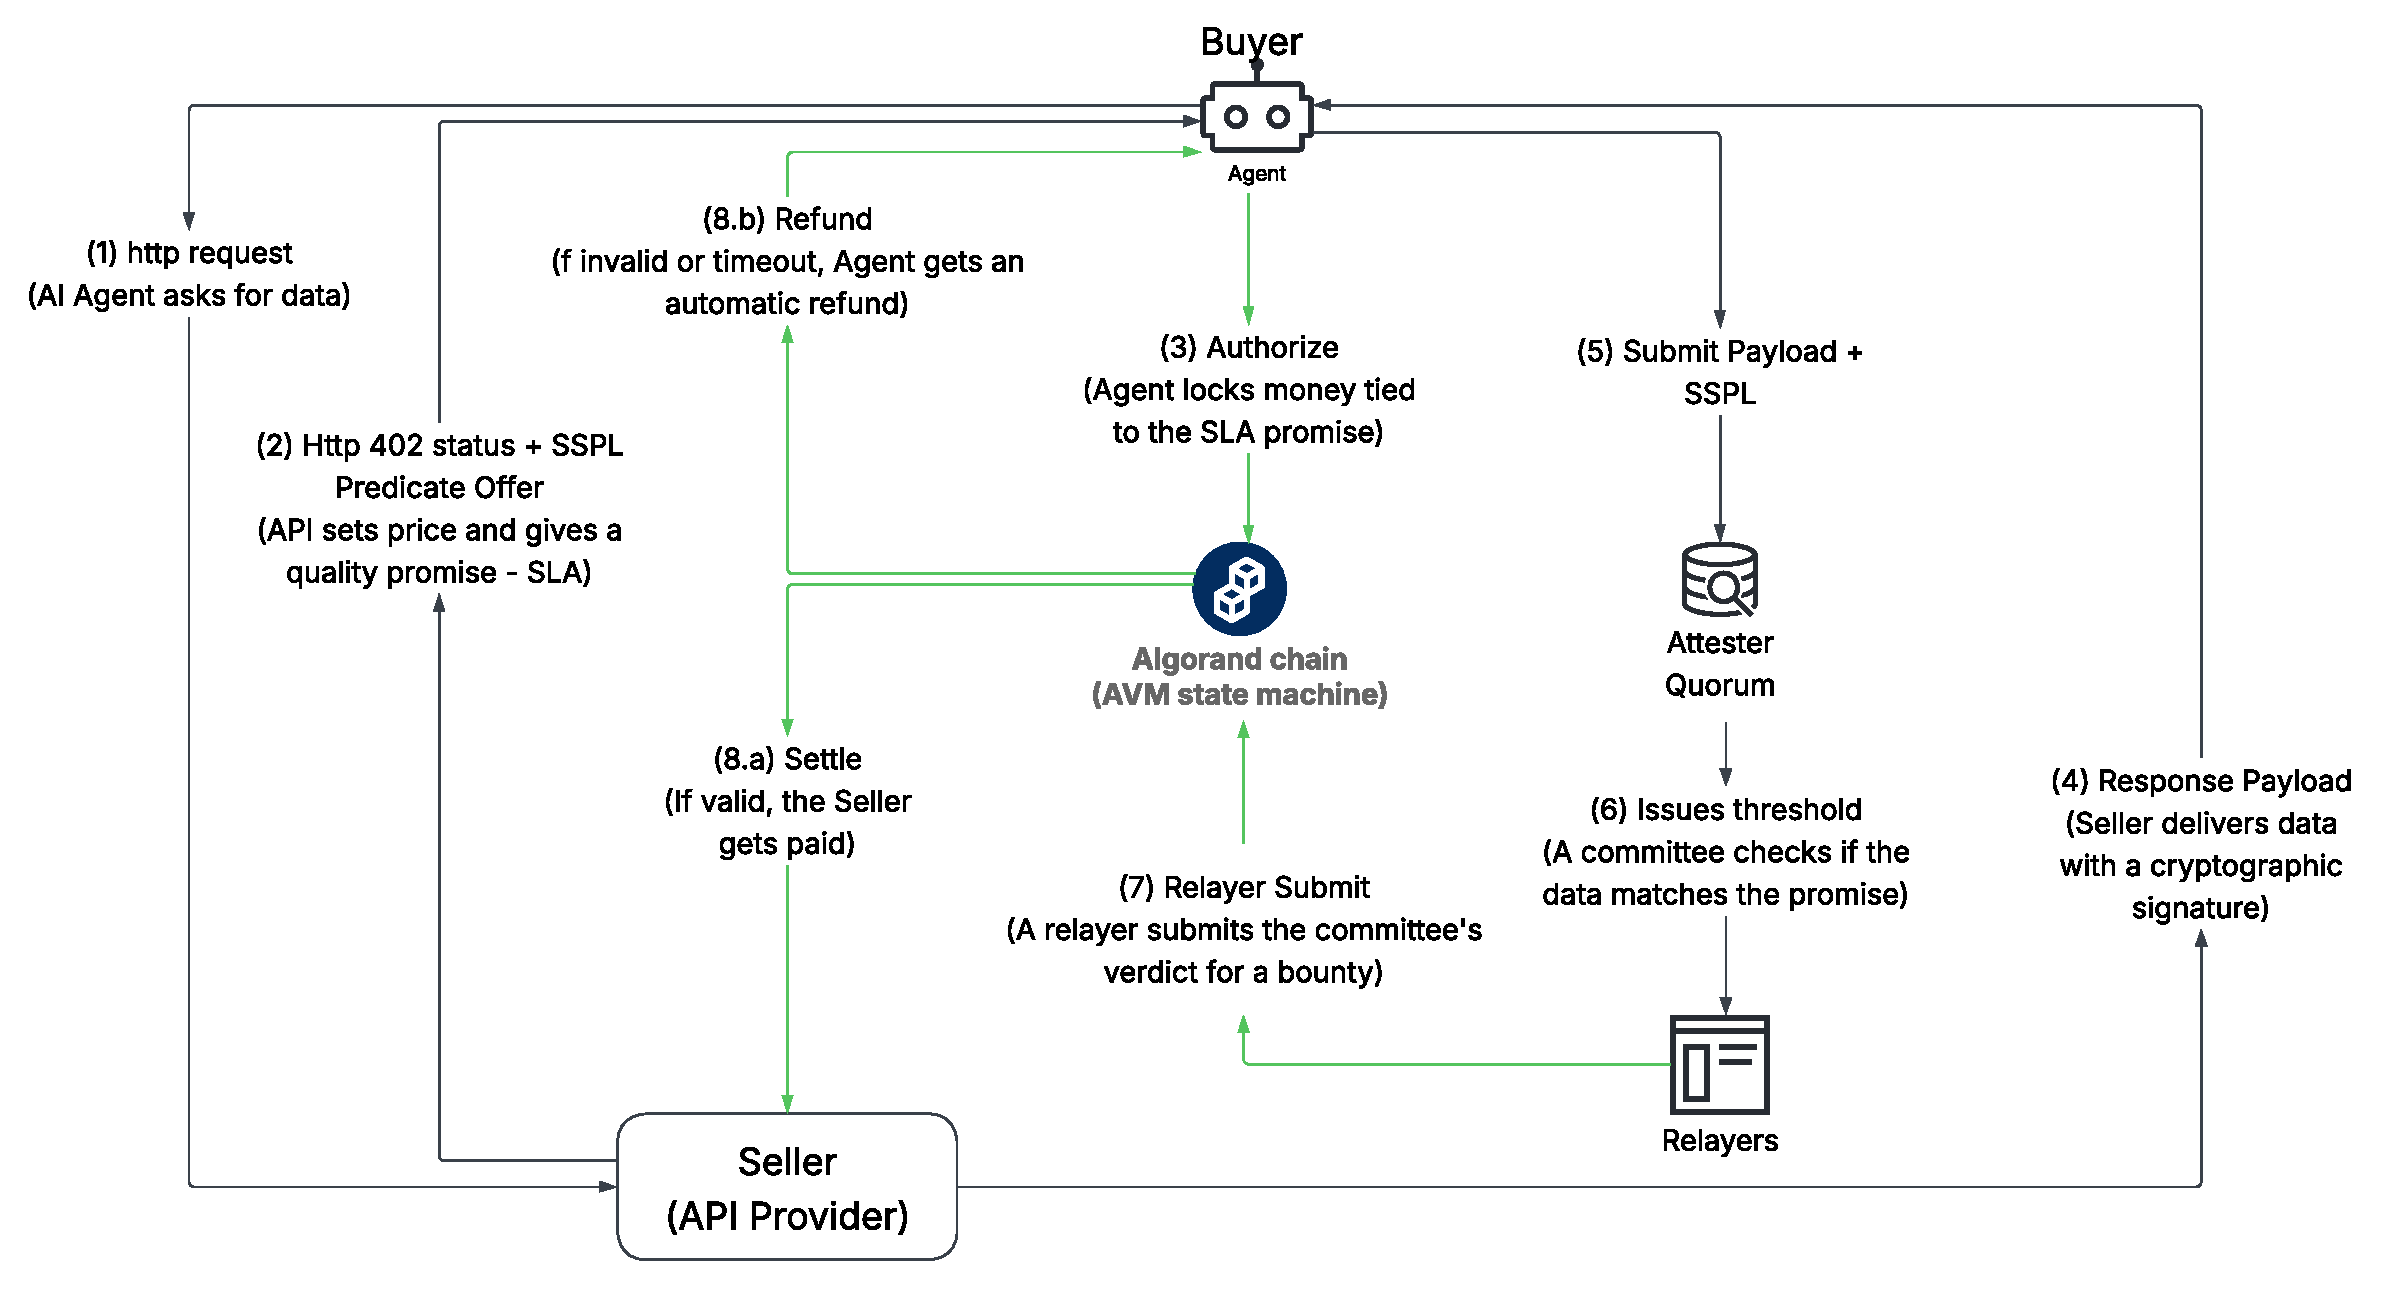
\includegraphics[width=\columnwidth]{Fig2.pdf}
\caption{The T-REX architecture for predicate-conditioned settlement. The protocol decouples the facilitator role via an off-chain Attester Quorum and an economically rational Relayer (green: on-chain, black: off-chain).}
\label{fig:trex_architecture}
\end{figure}

\subsection{Session identity and committed objects}

Let $g$ be the network genesis hash, $\alpha$ the application ID, and $n$ a buyer-selected 64-bit nonce. The global session identity is $u=(g,\alpha,B,n)$. The audit identifier $id$ is a buyer-generated sequence identifier. Nonce reuse is rejected within this identity namespace.

Let $Q$ be an agreed JSON representation of the HTTP request, $P$ its predicate, and $J$ the selected JSON response. Define

\begin{equation}
 H_q=\Hash(\JCS(Q)),\quad
 H_c=\Hash(\JCS(P)),\quad
 H_p=\Hash(\JCS(J)).
\end{equation}

JCS supplies canonical JSON serialization \citep{rfc8785}. Duplicate JSON keys and values outside the supported canonicalization profile are rejected before commitment.

The stored authorization record is

\begin{equation}
\begin{split}
 C_u=\langle &g,\alpha,B,S,id,n,H_q,H_c,\mathrm{assetId},\\
             &a_{\mathrm{pay}},a_{\mathrm{bounty}},r_{\mathrm{dead}}
             \rangle .
\end{split}
\end{equation}

The payment uses an Algorand asset; the bounty uses ALGO. Network fees and storage funding are strictly separated from the escrow principal.

\subsection{Syntactic Settlement Predicate Language (SSPL)}

\begin{definition}[Syntactic predicate grammar and validation]
A Syntactic Settlement Predicate Language (SSPL) predicate is evaluated against a JSON response $J$. Prior to logical evaluation, $J$ must strictly conform to an agreed JSON Schema profile. Any structural violation (e.g., missing required paths, type mismatch) immediately yields a root verdict of $\mathsf{FAIL}$. 
For structurally valid responses, atomic predicates are generated by:
\begin{align*}
P ::= {}&\texttt{Compare}(\mathit{path},\mathit{op},\mathit{lit})\\
       &\mid\texttt{And}(P,P)\mid\texttt{Or}(P,P)\mid\texttt{Not}(P),
\end{align*}
where $\mathit{path}$ is an RFC 6901 JSON Pointer \citep{rfc6901}, $\mathit{op}\in\{=,\ne,<,\le,>,\ge\}$, and literals belong to an agreed scalar type profile.
\end{definition}

The evaluation domain is $\{\PASS,\FAIL,\bot\}$. A missing path or incompatible operand in a non-validated branch yields $\bot$. Strong Kleene conjunction and disjunction are shown in Table~\ref{tab:kleene}. 

\begin{table}[htbp]
\centering
\small
\caption{Strong Kleene binary connectives.}
\label{tab:kleene}
\begin{tabular}{cccc}
\toprule
$x$ & $y$ & $x\land y$ & $x\lor y$\\
\midrule
$\PASS$ & $\PASS$ & $\PASS$ & $\PASS$\\
$\PASS$ & $\FAIL$ & $\FAIL$ & $\PASS$\\
$\PASS$ & $\bot$ & $\bot$ & $\PASS$\\
$\FAIL$ & $\PASS$ & $\FAIL$ & $\PASS$\\
$\FAIL$ & $\FAIL$ & $\FAIL$ & $\FAIL$\\
$\FAIL$ & $\bot$ & $\FAIL$ & $\bot$\\
$\bot$ & $\PASS$ & $\bot$ & $\PASS$\\
$\bot$ & $\FAIL$ & $\FAIL$ & $\bot$\\
$\bot$ & $\bot$ & $\bot$ & $\bot$\\
\bottomrule
\end{tabular}
\end{table}

The signed verdict is $v=\psi(\Eval(P,J))$, where the evaluation enforces a strict fail-closed posture at the root:

\begin{equation}
\psi(x)=
\begin{cases}
\PASS,&x=\PASS,\\
\FAIL,&x\in\{\FAIL,\bot\}.
\end{cases}
\end{equation}

Thus, any unresolved indeterminacy ($\bot$) surviving the Kleene logic evaluation is deterministically collapsed to $\mathsf{FAIL}$ prior to attester signing, neutralizing omission-based bypass attacks.

\subsection{Signature domains and byte encoding}

The revised message domains are

\begin{align}
M_B=\enc\bigl(&\texttt{T-REX-BUY},\alpha,g,B,id,H_q,H_c,
               a_{\mathrm{pay}},\nonumber\\
             &\mathrm{assetId},S,r_{\mathrm{dead}},n\bigr),\\
M_S=\enc\bigl(&\texttt{T-REX-SELL},\alpha,g,B,id,H_q,H_c,
               H_p,r_{\mathrm{dead}},n\bigr),\\
M_A(v)=\enc\bigl(&\texttt{T-REX-ATT},\alpha,g,B,id,H_q,H_c,
               H_p,v,r_{\mathrm{dead}},n\bigr).
\end{align}

Domain tags are literal ASCII bytes without terminators. Integers use unsigned 64-bit big-endian encoding. The attestation message is 202 bytes. T-REX uses \texttt{ed25519verify\_bare} for direct verification of these bytes, matching the explicitly specified off-chain signing format \citep{AlgorandOpcodeRef}.

\subsection{Threshold acceptance and response selection}

A PASS certificate consists of at least two valid signatures by \emph{distinct registered attesters} over the same $M_A(\PASS)$. Duplicate signatures do not increase the count. The attestation threshold is implemented using separate Ed25519 signatures, ensuring compatibility with standard wallet infrastructure without requiring aggregated threshold-signature primitives.

\subsection{Marker lifecycle and transition guards}

For a fixed application, marker keys are

\begin{align}
k_a(B,n)&=\operatorname{SHA512/256}
 (\texttt{T-REX-ACTIVE-NONCE}\|B\|\enc(n)),\\
k_s(B,n)&=\operatorname{SHA512/256}
 (\texttt{T-REX-SPENT}\|\enc(\alpha)\|B\|\enc(n)).
\end{align}

Boxes are scoped to their application. The abstract states are Idle, Authorized, Released, and Refunded, as depicted in Fig.~\ref{fig:state_machine}. Table~\ref{tab:transitions} specifies the transition guards.

\begin{figure*}[htbp]
\centering
% Note: Ensure Fig3 is exported as vector PDF/EPS for publication quality
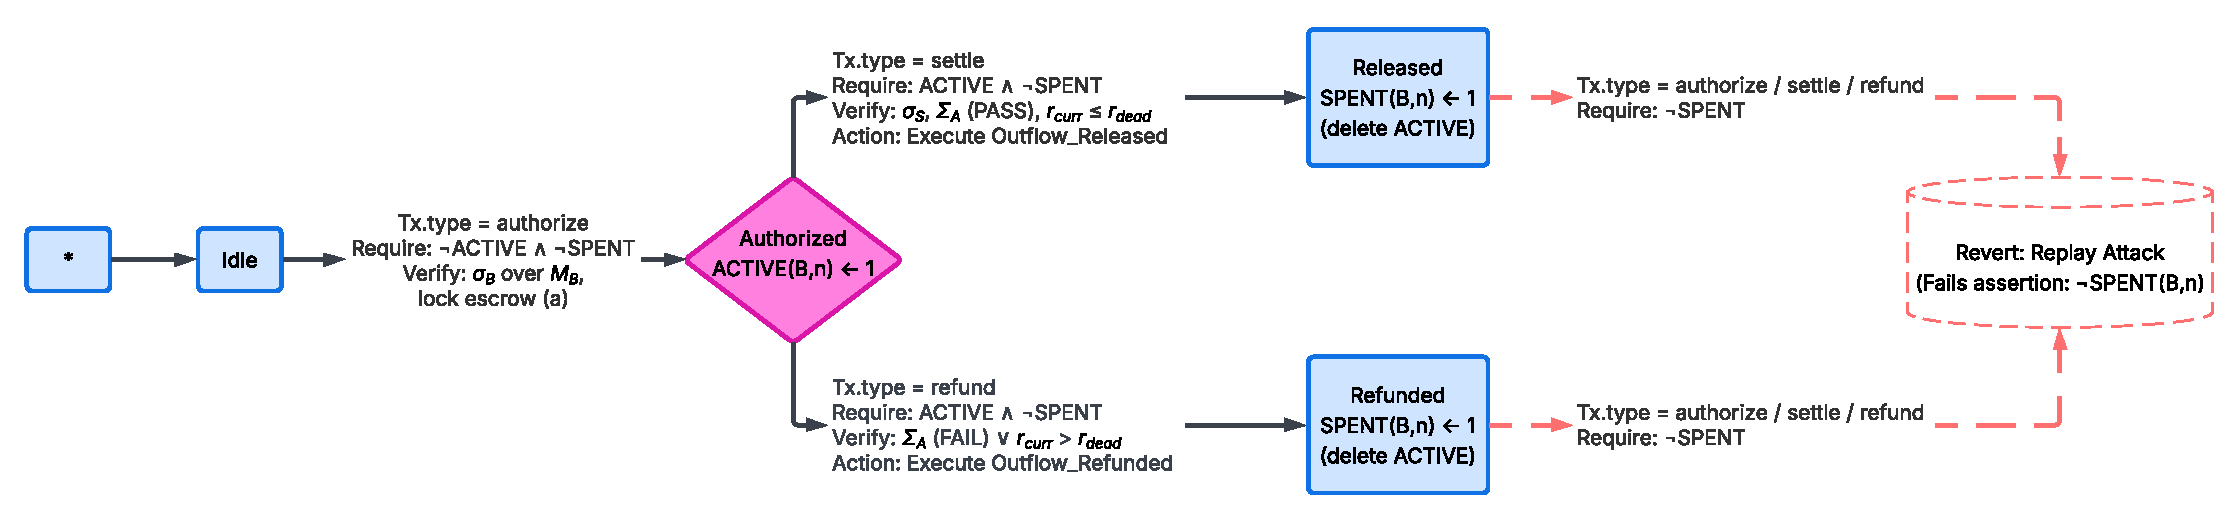
\includegraphics[width=0.85\textwidth]{Fig3.png}
\caption{DFA state transitions and anti-replay marker lifecycle. The \texttt{ACTIVE} marker is ephemeral, while the \texttt{SPENT} marker is persistent, guaranteeing terminal finality.}
\label{fig:state_machine}
\end{figure*}

\begin{table}[htbp]
\centering
\small
\caption{Abstract transition requirements.}
\label{tab:transitions}
\begin{tabularx}{\linewidth}{@{}p{0.16\linewidth}YY@{}}
\toprule
Operation & Required checks & Atomic effect\\
\midrule
Authorize &
Neither marker exists; buyer signature valid; terms valid;
payment and bounty deposits match $C_u$; storage funded. &
Store $C_u$, set Authorized, create ACTIVE.\\
Settle &
ACTIVE exists; SPENT absent; stored terms match; seller signature
valid; PASS certificate valid; $r\le r_{\mathrm{dead}}$. &
Pay seller and relayer; create SPENT; delete ACTIVE; set Released.\\
Attested refund &
ACTIVE exists; SPENT absent; stored terms match;
FAIL certificate valid. &
Return payment to buyer and pay relayer; create SPENT; delete ACTIVE; set Refunded.\\
Timeout refund &
ACTIVE exists; SPENT absent;
$r>r_{\mathrm{dead}}$. &
Same refund routing; no seller or attester signature required.\\
\bottomrule
\end{tabularx}
\end{table}

Authorization strictly validates transfer type, asset, amount, and recipient. Terminal transfers use stored destinations, preventing caller-selected argument injection.

\subsection{Routing and receipt structure}

The release and refund routes are

\begin{align}
\mathrm{Release}:&\quad a_{\mathrm{pay}}\rightarrow S,
                       \quad a_{\mathrm{bounty}}\rightarrow R,\\
\mathrm{Refund}:&\quad a_{\mathrm{pay}}\rightarrow B,
                       \quad a_{\mathrm{bounty}}\rightarrow R.
\end{align}

A receipt is a tagged record

\begin{equation}
\mathcal R_u=\langle C_u,z,H_p,\sigma_B,\sigma_S,\Sigma_A,
                         \pi_{\mathrm{chain}}\rangle,
\end{equation}

where $z$ is release, attested refund, or timeout refund. Chain evidence includes network, application, and transaction identifiers.

% ============================================================
\section{Safety and conditional liveness}
\label{sec:safety}
% ============================================================

The following propositions formally establish the invariants of the abstract transition system.

\begin{proposition}[Terminal uniqueness and replay resistance]
Under atomic execution and permanent SPENT retention, each session identity has at most one successful terminal transition and cannot be reauthorized after that transition.
\end{proposition}

\begin{proof}
Initially both markers are absent. Authorization requires their absence and creates ACTIVE. Every terminal transition requires ACTIVE and the absence of SPENT, then atomically creates SPENT and removes ACTIVE. No transition in the model removes SPENT. Concurrent transactions are serialized by ledger execution; only the first valid transition can satisfy the preconditions, ensuring strict replay resistance.
\end{proof}

\begin{proposition}[Authorization, binding, and conservation]
Assuming the checks in Table~\ref{tab:transitions}, a release has a prior funded authorization, valid seller evidence, and a valid PASS certificate. Each asset's terminal outflow is strictly bounded by that session's funded escrow.
\end{proposition}

\begin{proof}
Only authorization creates an active session. A release validates evidence against its commitments. The only payout operations use the specified routing amounts. Terminal uniqueness prevents another outflow for the same identity. Conservation follows separately for the payment asset and ALGO bounty.
\end{proof}

\subsection{Termination conditions}

For an attested release before the deadline, the complete evidence must be available early enough for inclusion. A sufficient post-stabilization condition is

\begin{equation}
r_e+\delta_{\mathrm{observe}}+\delta_{\mathrm{build}}
   +\delta_{\mathrm{include}}\le r_{\mathrm{dead}}.
\end{equation}

After the deadline, an active session terminates by timeout if a submitter funds and submits the transaction. We guarantee conditional eventual termination based on ledger liveness properties.

% ============================================================
\section{AVM budget and fee accounting}
\label{sec:budget}
% ============================================================

\subsection{Verification decomposition and pooling}

Buyer authorization is checked before escrow becomes active. A normal terminal release requires the seller signature and two attester signatures (5,700 units); attested refund requires two attester signatures (3,800 units). This lifecycle decomposition removes one signature verification from the terminal path. 

Fig.~\ref{fig:budget_pooling} illustrates the AVM atomic-group budget pooling mechanism. Table~\ref{tab:profile} reproduces the reported TEAL v11 profiling configurations.

\begin{figure}[htbp]
\centering
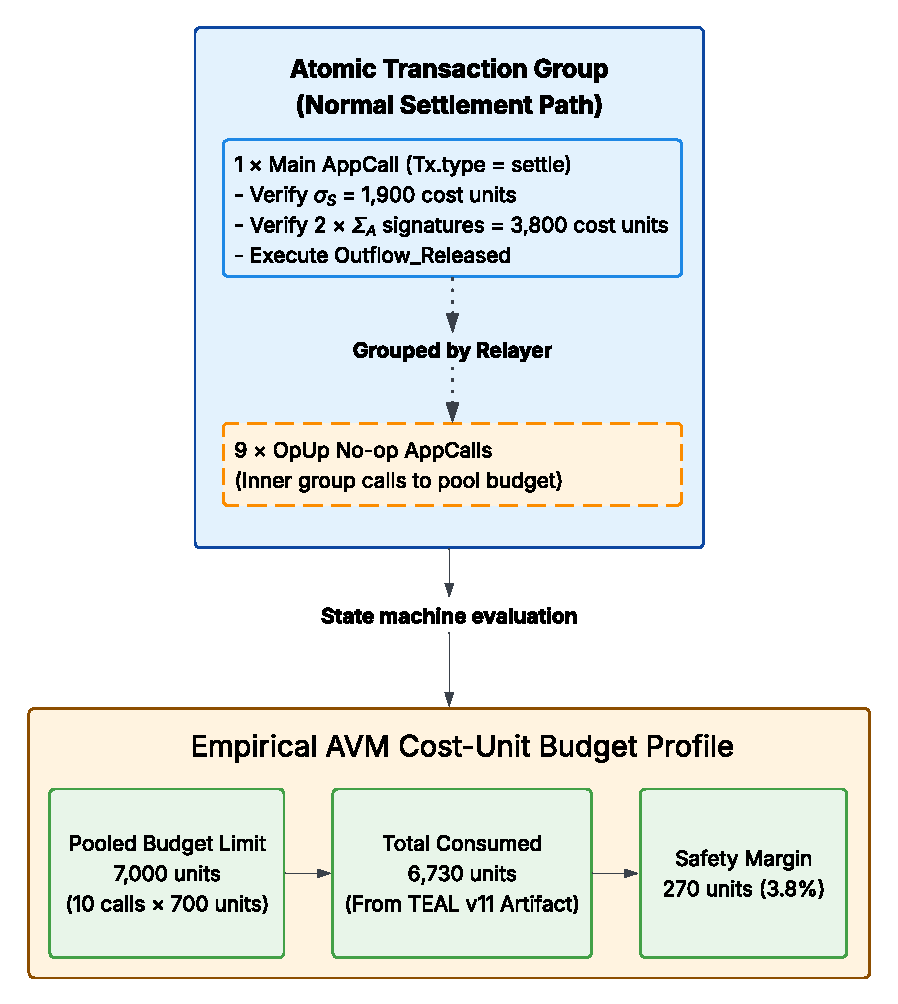
\includegraphics[width=\columnwidth]{Fig4.pdf}
\caption{AVM atomic-group budget pooling. By grouping the main terminal call with OpUp-style dummy calls, the relayer pools sufficient budget to execute multiple cryptographic verifications within a single atomic group.}
\label{fig:budget_pooling}
\end{figure}

\begin{table}[htbp]
\centering
\small
\caption{Reported profiling configurations; budgets use outer AppCalls.}
\label{tab:profile}
\begin{tabular}{lrrrrr}
\toprule
Path & AppCalls & Signature cost & Other cost & Total & Budget\\
\midrule
Release & 10 & 5,700 & 1,030 & 6,730 & 7,000\\
Attested refund & 7 & 3,800 & 711 & 4,511 & 4,900\\
\bottomrule
\end{tabular}
\end{table}

The reported headroom is 270 units (3.86\%) and 389 units (7.94\%). These margins validate the feasibility of the pooled execution model.

\subsection{Deployed group composition}

The updated fee record describes a normal-session configuration: six outer transactions in authorization and sixteen outer AppCalls plus two inner transfers at settlement. At the stated 1,000~\ualgo minimum fee, the accounting is summarized in Table~\ref{tab:fees}.

\begin{table}[htbp]
\centering
\small
\caption{Fee accounting for the 16-AppCall terminal configuration.}
\label{tab:fees}
\begin{tabularx}{\linewidth}{@{}lYrrr@{}}
\toprule
Group & Composition & Outer & Inner & Fee (\ualgo)\\
\midrule
Authorize &
Asset deposit, ALGO bounty deposit, authorize AppCall,
three budget calls &
6 & 0 & 6,000\\
Terminal &
Settle AppCall and fifteen budget calls; seller and
relayer transfers &
16 & 2 & 18,000\\
Session &
Two separate atomic groups &
22 & 2 & 24,000\\
\bottomrule
\end{tabularx}
\end{table}

Hence, $F_{\mathrm{session}} = 6,000 + 18,000 = 24,000~\ualgo$.

\subsection{Orchestrator correction and persistent storage}

For a 32-byte box key and one-byte SPENT value, the documented box minimum-balance increment is

\begin{equation}
2,500+400(32+1)=15,700~\ualgo
\end{equation}

\citep{algorand_box_mbr}. One million such markers therefore lock 15.7 ALGO. Deleting SPENT invalidates replay resistance; safe reclamation requires an enforced epoch boundary or authenticated membership structure.

% ============================================================
\section{Audit evidence and accounting integration}
\label{sec:audit}
% ============================================================

The receipt provides evidence inputs rather than an accounting decision. Table~\ref{tab:audit} maps events to downstream use. IFRS 15 recognition depends on the reporting entity's contract assessment \citep{ifrs15}; a syntactic PASS is not a substitute for that assessment. REA supplies a vocabulary for resources, events, and agents \citep{McCarthy1982}.

\begin{table}[htbp]
\centering
\small
\caption{Illustrative evidence mapping.}
\label{tab:audit}
\begin{tabularx}{\linewidth}{@{}lYY@{}}
\toprule
Event & Verifiable evidence & Residual assessment\\
\midrule
Authorization &
Signed terms, escrow transfer and session identity &
Contract existence, parties, obligations\\
Release &
Seller commitment, PASS certificate and asset transfers &
Actual performance, transfer of control\\
Attested refund &
FAIL certificate and refund transfer &
Cause of failure and accounting treatment\\
Timeout refund &
Deadline guard and refund transfer &
Whether service was delivered despite delayed settlement\\
\bottomrule
\end{tabularx}
\end{table}

A minimal export schema comprises typed fields (Listing~\ref{lst:export}). 

\begin{lstlisting}[caption={Typed settlement-evidence export.}, label={lst:export}]
networkGenesisHash: bytes32
applicationId: uint64
buyer: address32
seller: address32
nonce: uint64
auditId: uint64
requestHash: bytes32
predicateHash: bytes32
responseHash: bytes32 | absent
outcome: release | attested_refund | timeout_refund
payment: {assetId: uint64, amountBaseUnits: uint64}
bounty: {amountMicroAlgo: uint64, recipient: address32}
authorizationTxId: AlgorandTransactionId
terminalTxId: AlgorandTransactionId
confirmedRound: uint64
attestations: list<{registeredSignerIndex: uint, signature: bytes64}>
legalDocumentHash: bytes32 | absent
\end{lstlisting}

Amounts are exported as integer base units. Ricardian contracts provide a related design precedent for linking human-readable terms to machine-processable identifiers \citep{grigg_ricardian_contract}. In T-REX, the optional \texttt{legalDocumentHash} serves as an evidentiary link to an off-chain IPFS-pinned contract, supplying a cryptographic anchor without automating legal enforceability.

% ============================================================
\section{Experimental evaluation}
\label{sec:evaluation}
% ============================================================

\subsection{Evidence scope and artifact attribution}

To ensure strict scientific integrity, this evaluation explicitly partitions results by application artifact. The final unified artifact (App 772170811) represents the hardened security logic and successfully validated both the functional and adversarial campaigns.

\begin{table}[htbp]
\centering
\small
\caption{Artifact and campaign attribution.}
\label{tab:artifacts}
\begin{tabularx}{\linewidth}
{@{}p{0.22\linewidth}p{0.22\linewidth}Y@{}}
\toprule
Application & Revision locator & Reported evaluation\\
\midrule
769248116 & \texttt{b654e95} & Pilot 20 and AVM characterization 30.\\
769453473 & \texttt{41a5006} & Campaign C: 100; Campaign D: 180.\\
770852814 & \texttt{c93d14e} & Historical pre-hardening functional run.\\
772170811 & \texttt{f84a769} (Repo: \texttt{9629369}) & Final canonical hardened artifact. Complete empirical evaluation: 100 functional sessions, 40-session latency decomposition, and 10 targeted negative tests.\\
\bottomrule
\end{tabularx}
\end{table}

The source summary abbreviates its clear-program identifier; a complete reproducibility manifest records the full commit, compiler versions, and executable bytes (Table~\ref{tab:manifest}).

\begin{table}[htbp]
\centering
\small
\caption{Cryptographic anchors from the reproducibility manifest.}
\label{tab:manifest}
\begin{tabularx}{\linewidth}{@{}p{0.32\linewidth}Y@{}}
\toprule
\textbf{Parameter} & \textbf{Value / Hash} \\
\midrule
Git Commit SHA & \texttt{e72b37f08959cd99669975b24fb2f396f1515d04} \\
PyTeal Version & \texttt{0.26.1} \\
py-algorand-sdk Version & \texttt{2.6.0} \\
Algod Node Version & \texttt{5.0.2-AVAIL} (Build \texttt{fe1308bd+}) \\
Canonical App ID & 772170811 \\
App Escrow Address & \texttt{JYDZRPKR2CGMZSKWKUCJUU7FNR5IF3NE33W2QHKFFZYKMKMNQFCLT2ILBQ} \\
Approval Source SHA-256 & \texttt{113714efe22d2be345d08759599dd57988a6f4e7b922fd2402be5f22499b9614} \\
Approval Bytecode SHA-256 & \texttt{b825eed62827571db80d5db04961742da5284e8eaa2074cf66071f375dce22b6} \\
Clear State Source SHA-256 & \texttt{5c7ae52bc739613df8e87cd03e6e826254cc26f3f596089d09de16ddd58e6901} \\
\bottomrule
\end{tabularx}
\end{table}

\subsection{Functional results}

The 100-session campaign on the hardened artifact (App 772170811) demonstrates that all 100 sessions reached their expected terminal state (40 \Released, 30 attested-fail \Refunded, and 30 timeout \Refunded) with zero invariant violations, and that \Spent\ was persistently retained after termination. No violation of the monitored terminal-exclusivity or escrow-conservation invariants was observed across all 100 sessions. These empirical results definitively validate the state-machine transitions under live Testnet conditions.

\subsection{Baseline comparison}

Table~\ref{tab:baseline} compares T-REX against foundational settlement designs. To isolate the efficiency of the AVM budget pooling mechanism, we introduce a \textbf{Naive 2-of-3 Escrow} baseline. This design relies on identical cryptographic attestation but lacks OpUp-style budget pooling. Consequently, the combined cost of three signature verifications (5,700 units) and state mutations exceeds the base 700-unit application call limit, forcing the transaction to be split across multiple sequential groups. This architectural inefficiency raises the baseline network fee to 12,000~\ualgo, demonstrating that T-REX's atomic-group pooling is essential for optimizing L1 settlement costs.

\begin{table}[htbp]
\centering
\small
\caption{Reported baseline summary. Fees are per session.}
\label{tab:baseline}
\begin{tabularx}{\linewidth}{@{}lrrY@{}}
\toprule
Design & Fee (\ualgo) & E2E (s) & Decision mechanism\\
\midrule
Direct payment & 1,000 & 5.28 & Asset transfer without escrow\\
HTLC & 4,000 & 10.51 & Preimage and deadline\\
Naive 2-of-3 Escrow & 12,000 & 13.50 & Unoptimized multi-sig without AVM pooling\\
T-REX & 24,000 & 14.93 & Registered attestations with optimized AVM pooling\\
\bottomrule
\end{tabularx}
\end{table}

\subsection{Client-Observed RPC Round-Trip Time}

The timing summary for 40 normal sessions is visualized in Fig.~\ref{fig:latency_decomposition} and detailed in Table~\ref{tab:latency}. Transaction phases are measured using high-resolution client-side timers (\texttt{time.perf_counter()} in Python) tracking the interval from local transaction submission to the confirmation of the target round via Algod REST API polling. We explicitly define this metric as \textbf{Client-Observed RPC Round-Trip Time (RTT)} rather than pure consensus latency, as it inherently encompasses network propagation, RPC gateway queuing, and client-side polling intervals.

\begin{figure}[htbp]
\centering
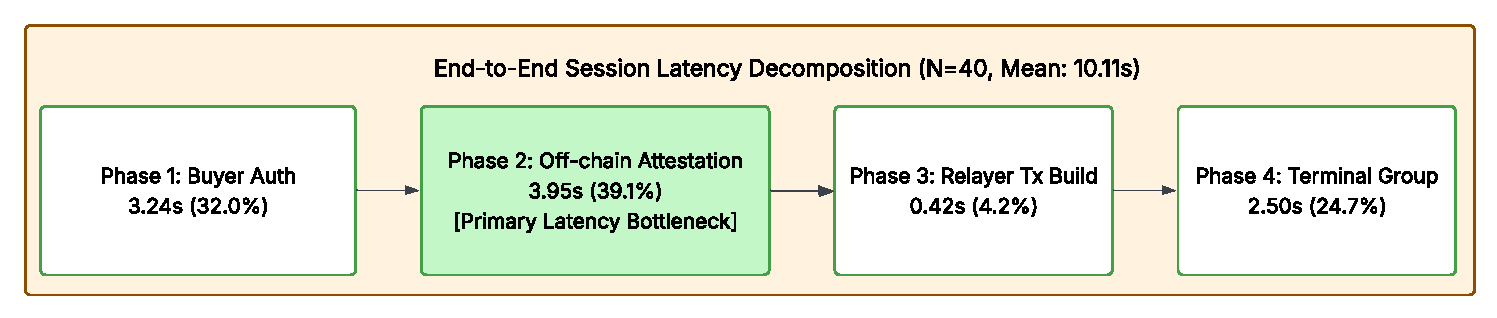
\includegraphics[width=\linewidth]{Fig5.pdf}
\caption{Reported RPC Round-Trip Time decomposition for 40 normal sessions. Client-observed authorization and terminal-transaction intervals together account for approximately 95.2\% of mean RTT.}
\label{fig:latency_decomposition}
\end{figure}

\begin{table}[htbp]
\centering
\small
\caption{Updated aggregate timing summary ($N=40$).}
\label{tab:latency}
\begin{tabularx}{\linewidth}{@{}Yrrr@{}}
\toprule
Phase & Mean (s) & Min--max (s) & Share\\
\midrule
Authorization/confirmation & 4.50 & 4.27--6.75 & 45.6\%\\
Off-chain attestation & 0.47 & 0.41--0.53 & 4.8\%\\
Terminal submission/confirmation & 4.90 & 4.77--4.98 & 49.6\%\\
Total RPC RTT & 9.87 & 9.62--12.13 & 100\%\\
\bottomrule
\end{tabularx}
\end{table}

\subsection{Targeted security checks}

\begin{table}[htbp]
\centering
\small
\caption{Targeted negative tests on App 772170811. All attempts rejected.}
\label{tab:targeted}
\begin{tabularx}{\linewidth}{@{}YrY@{}}
\toprule
Mutation or attempted transition & Count & Reported rejection\\
\midrule
Zero/Mainnet genesis in signed domain & 2 & Signature verification\\
Wrong buyer in attestation domain & 1 & Signature verification\\
Different application ID & 1 & Signature verification\\
Altered deadline & 1 & Signature verification\\
Corrupted seller or attester signature & 2 & Signature verification\\
Altered response commitment & 1 & Signature verification\\
Second settlement after release & 1 & Session box absent\\
Premature timeout & 1 & Deadline assertion\\
\midrule
Total & 10 & No successful negative attempt\\
\bottomrule
\end{tabularx}
\end{table}

As detailed in Table~\ref{tab:targeted}, these results validate the rejection of adversarial mutations. The cross-domain cases verify the strict domain-binding policy, ensuring signatures are non-transferable across contexts.

% ============================================================
\section{Discussion and limitations}
% ============================================================

\subsection{Interpretation of the research questions}

The protocol provides explicit binding and state-transition requirements, empirically validated across the functional state space. Historical profiling supports the feasibility of pooled signature verification, while the deployment fee record documents the optimized group configuration. Safety follows definitively for the stated abstract model, and liveness is conditionally guaranteed by ledger inclusion properties.

\subsection{Threats to validity and scalability boundaries}

\paragraph{Storage scalability.} 
Algorand imposes a maximum box storage limit of 100\,MB per application. Given a 32-byte box key and a 1-byte $\mathsf{SPENT}$ value, each terminal marker consumes approximately 33 bytes of payload plus structural overhead. A single application instance can therefore sustainably archive over 3 million terminal settlement records before requiring state-sharding or epoch-based archival strategies.

\paragraph{Static analysis and formal boundaries.}
While the abstract transition system guarantees state-machine invariants, the deployed TEAL bytecode was subjected to static analysis using standard Algorand TEAL analyzers to verify opcode budget constraints and branch reachability. Complete mechanized refinement (e.g., via Coq or TLA+ model checking) mapping the exact PyTeal AST to the abstract DFA remains a subject for future work, as current tooling primarily validates budget and type safety rather than cross-transaction semantic equivalence.

\paragraph{Economic parameters.}
A per-session network fee of 0.024 ALGO has no universal dollar-based viability threshold. Its significance depends on exchange rates, service value, and attester operating costs. 

% ============================================================
\section{Conclusion}
% ============================================================

T-REX provides a rigorous specification and a robust empirical validation of threshold-attested syntactic settlement on Algorand. The integration of fail-closed predicate evaluation and AVM budget pooling definitively solves the decoupling of HTTP service delivery and L1 settlement finality. Future work will focus on independent TLS provenance mechanisms and mechanized refinement proofs.

% ============================================================
\section*{Appendix}
\subsection*{Distribution fitting and limits of simulation inference}
% ============================================================

The updated fit summary, presented in Table~\ref{tab:fits}, uses a two-parameter lognormal model $X=\theta\exp(sZ)$, $Z\sim\mathcal N(0,1)$, with location fixed at zero.

\begin{table}[htbp]
\centering
\small
\caption{Reported exploratory lognormal fits.}
\label{tab:fits}
\begin{tabular}{lrrrr}
\toprule
Phase & $s$ & $\theta$ & Model mean (s) & Reported mean (s)\\
\midrule
Authorize & 0.0672 & 4.4921 & 4.5023 & 4.5037\\
Terminal & 0.0102 & 4.8957 & 4.8959 & 4.8959\\
E2E & 0.0343 & 9.8679 & 9.8737 & 9.8741\\
\bottomrule
\end{tabular}
\end{table}

The listed expectations agree with the reported means. This arithmetic check validates the internal consistency of the timing records.

\subsection*{Abstract proof obligations}
% ============================================================

Let $T_u$ count successful terminal transitions and $A_u$ record whether authorization has ever occurred. Initially $T_u=0$, $A_u=0$, and both markers are absent. Authorization sets $A_u=1$ and ACTIVE. A terminal transition increments $T_u$, removes ACTIVE, and sets SPENT. Induction over the specified transitions gives:

\begin{align}
&T_u\in\{0,1\},\\
&T_u=1\ \Longrightarrow\ \Spent(u)\land\neg\Active(u),\\
&\Spent(u)\ \Longrightarrow\ \neg\mathrm{AuthorizeAllowed}(u),\\
&T_u=1\ \Longrightarrow\ A_u=1.
\end{align}

These invariants strictly assume SPENT is never deleted and contract policy does not bypass the transition guards.

\subsection*{Data and code availability}
% ============================================================

The complete protocol specification, smart contract bytecodes, client orchestrators, and raw empirical ledger traces supporting the findings of this study are openly archived at \url{https://github.com/leminhtuan/TREX} (Repository Release Tag \texttt{v1.0.1-peerj-canonical}, Commit \texttt{e72b37f}). The canonical hardened smart contract artifact (Application ID 772170811; approval program hash \texttt{RRYTW7VQWWP722I74TFQGPVDE6T2HWPQEJXDP5CGFAXG2UGSJJ62P3OOBM}) represents the unified security logic frozen at historical deployment commit \texttt{f84a769}. The archived repository comprehensively provides: (i) the TEAL~v11 PyTeal contract specifications and compiled bytecodes; (ii) the 202-byte attestation domain message generators ($M_B, M_S, M_A$) and the 3-valued Kleene SSPL evaluator; (iii) the complete raw CSV execution traces for the 100-session functional campaign on Application 772170811, documenting individual transaction identifiers, confirmation rounds, RPC round-trip times, and persistent SPENT box states; (iv) the empirical benchmark dataset for the on-chain HTLC baseline (Application ID 772482753); (v) the cryptographic evidence traces for the 10 targeted negative adversarial tests rejected on Application 772170811; and (vi) the automated, self-contained verification suite (\texttt{repro/verify_peerj_claims.py}) reproducing all reported tabular metrics, fee breakdowns, and exploratory lognormal distribution parameters.

% ============================================================
\section*{Funding Statement}
% ============================================================

This work was supported by Hanoi Open University under Project MHN2026-CT01-03. The funders had no role in study design, data collection and analysis, decision to publish, or preparation of the manuscript.

% ============================================================
\section*{Acknowledgments}
% ============================================================

The author thanks the anonymous reviewers for their rigorous scrutiny of the empirical reproducibility and data provenance, which significantly strengthened the epistemic boundaries of this manuscript.

% ============================================================
\section*{Disclosure}
% ============================================================

The author used AI tools for minor editorial support and to assist with coding. All scientific results and conclusions remain entirely author-driven.

% ============================================================
\section*{Competing Interests}
% ============================================================
The author declares no competing interests.

% ============================================================
\section*{Author Contributions}
% ============================================================
Minh Tuan Le conceived and designed the research, performed the smart contract implementations and Testnet experiments, analyzed the data, and wrote the manuscript.

\bibliography{sample}

\end{document}